\documentclass[%
%reprint,
superscriptaddress,
%groupedaddress,
%unsortedaddress,
%runinaddress,
%frontmatterverbose,
%preprint,
showpacs,
%preprintnumbers,
nofootinbib,
%nobibnotes,
%bibnotes,
amsmath,amssymb,
aps,
%pra,
%prb,
prc,
%paper,
%rmp,
%prstab,
%prstper,
twocolumn,
floatfix ]%
{revtex4-1}

%\usepackage{acrofont}%NOTE: Comment out this line for the release version!
\newcommand{\revtex}{REV\TeX\ }
\newcommand{\classoption}[1]{\texttt{#1}}
\newcommand{\macro}[1]{\texttt{\textbackslash#1}}
\newcommand{\m}[1]{\macro{#1}}
\newcommand{\env}[1]{\texttt{#1}}
\setlength{\textheight}{9.5in}

\usepackage{comment}
\usepackage[dvips]{graphicx}
%\usepackage{amsmath,amssymb}
%\usepackage{mathrsfs}
%\usepackage{txfonts}
\usepackage{braket}
%\usepackage{latexsym}
%\usepackage{ascmac}
%\usepackage{fancybox}
%\usepackage{type1cm}
\usepackage{cases}
\usepackage{caption}
%\usepackage[top=25truemm,bottom=20truemm,left=20truemm,right=20truemm]{geometry}

  \makeatletter
    \renewcommand{\theequation}{%
    \thesection.\arabic{equation}}
    \@addtoreset{equation}{section}
  \makeatother

\begin{document}

\renewcommand{\thefootnote}{\fnsymbol{footnote}}

\title{Low-lying collective excited states in non-integrable pairing models
based on stationary phase approximation to the path integral}%

\author{Fang Ni}
 \affiliation{Faculty of Pure and Applied Sciences,
              University of Tsukuba, Tsukuba 305-8571, Japan}
\author{Nobuo Hinohara}
 \affiliation{Faculty of Pure and Applied Sciences,
              University of Tsukuba, Tsukuba 305-8571, Japan}
 \affiliation{Center for Computational Sciences,
              University of Tsukuba, Tsukuba 305-8577, Japan}
\author{Takashi Nakatsukasa}
 \affiliation{Faculty of Pure and Applied Sciences,
              University of Tsukuba, Tsukuba 305-8571, Japan}
 \affiliation{Center for Computational Sciences,
              University of Tsukuba, Tsukuba 305-8577, Japan}
 \affiliation{iTHES Research Group, RIKEN, Wako 351-0198, Japan}

\begin{abstract}
For a description of large amplitude collective motion associated with
nuclear pairing, requantization of time-dependent mean-field dynamics
is performed using the stationary phase approximation (SPA) to the path
integral.
A disadvantage of the SPA is that it is applicable only to integrable systems.
We overcome this difficulty by developing a requantization approach
combining the SPA with the adiabatic
self-consistent collective coordinate method (ASCC+SPA).
We apply the theoretical framework of ASCC+SPA to 
a multi-level pairing models, which is non-integrable systems,
to study the nuclear pairing dynamics.
The ASCC+SPA gives a reasonable description of low-lying excited $0^+$
states in non-integrable pairing systems.
%\begin{description}
%\item[Background] This part would describe the
%context needed to understand what the paper
%is about.
%\item[Purpose] This part would state the purpose
%of the present paper.
%\item[Method] This part describe the methods
%used in the paper.
%\item[Results] This part would summarize the
%results.
%\item[Conclusions] This part would state the
%conclusions of the paper.
%\end{description}
\end{abstract}

\maketitle

\section{Introduction}
%pairing in nuclei
Pairing correlation plays an important role in open-shell nuclei.
Effect of the pairing is prominent in many observables for the ground states,
such as odd-even mass difference, moment of inertia of rotational bands,
and common quantum number $J^\pi=0^+$ for even-even nuclei \cite{RS80}.
Elementary excitations associated with the pairing,
pairing vibrations and pairing rotations,
have been observed in a number of nuclei \cite{BB05}.
Most of these states, ``excited'' from neghboring even-even systems,
are associated with the ground $J^\pi=0^+$ states in even-even nuclei.
In contrast, properties of excited $J^{\pi}=0^+$ states are not clearly
understood yet \cite{HW11, G01}, for which the pairing dynamics plays
an important role in a low-energy region (a few MeV excitation) of nuclei. 
In this paper,
we aim to understand the dynamics from pairing correlation in nuclei
from microscopic view point.

%TDMF theory and ASCC
The time-dependent mean-field (TDMF) theory is a standard theory to describe
the dynamics of nuclei from the microscopic degrees of freedom.
Inclusion of the pairing dynamcs leads to the
time-dependent Hartree-Fock-Bogoliubov (TDHFB) theory,
which has been utilized for a number of studies of nuclear reaction
and structure \cite{NMMY16}.
The small-amplitude approximation of TDHFB with modern energy density
functionals, quasiparticle random phase approximation (QRPA), 
has successfully reproduced properties of giant resonances in nuclei.
In contrast, the QRPA description of low-lying quadrupole vibrations
is not as good as the giant resonances \cite{NMMY16}.
A large-amplitude nature of the quantum shape fluctuation is supposed to
be important for these low-lying collective states.
Five-dimensional collective Hamiltonian (5DCH) approaches
have been developed for studies of low-lying quadrupole states,
in which the collective Hamiltonian is constructed from
microscopic degrees of freedom using the mean-field calculation and
the cranking inertia formula \cite{Bar11,Del10,Fu13}.
The 5DCH model is able to take into account fluctuations of
the quadrupole shape degrees of freedom which are important in many
nuclear low-energy phenomena, such as
shape coexistence and anharmonic quadrupole vibration.
However, the calculated inertia is often too small to reproduce
experimental data, due to the lack of time-odd components
in the cranking formula \cite{RS80}.
This deficiency can be remedied in the adiabatic self-consistent collective
coordinate (ASCC) method \cite{MNM00},
in which the time-odd effect is properly treated.
In addition, the ASCC method enables us to identify a collective subspace
of interest.
The ASCC was developed from the basic idea of self-consistent
collective coordinate method (SCC) by Marumori and coworkers \cite{MMSK80}.
It has been applied to the nuclear quadrupole dynamics including
the shape coexistence \cite{KNMM05, HNMM07, HNMM08}.
%A state in the collective subspace corresponds to a microscopic state
%in TDHFB phase space connected by $Q$ and $P$ operators in ASCC. 

%previous work
TDMF (TDHFB) theory corresponds to an SPA solution in the path integral
formulation \cite{Neg82}.
It lacks a part of quantum fluctuation
important in the large amplitude dynamics.
To introduce the quantum fluctuation based on the TDHFB theory,
the requantization is necessary \cite{Neg82,L80,LNP80,Rei80,KS80,K81}.
A simple and straightforward way of requantization is
the canonical quantization.
This is extensively utilized for collective models in nuclear physics.
For instance,
the canonical quantization of the 5DCH was employed for the study of low-lying
excited states in nuclei \cite{PR09,HSNMM10,NMMY16}.
The similar quantization was also utilized for the pairing collective
Hamiltonian \cite{BBPK70, GPBW85, ZPPRS99, P07}.
%However, the Hilbert space which the wave function obtained from canonical quantization belongs to is quite different from the Hilbert space which the original wave function belongs to. It may cause the deviation for the requantized states. 
In our previous work \cite{NN18},
we studied various requantization methods for the two-level pair model,
to investigate low-lying excited $0^+$ states.
Since the collectivity is rather low in the pairing motion in nuclei,
the canonical quantization often fails to produce an approximate answer
to the exact solution.
In contrast,
the stationary phase approximation (SPA) to the path integral \cite{SM88} 
can give quantitative results not only for the excitation energies, 
but also for the wave functions and two-particle-transfer strengths.
%We confirmed that SPA is superior to canonical requantization, especially for the calculation of two-particle transitional strength. 
The quantized states obtained in the SPA has two advantages:
First, the wave functions are given directly in terms of
the microscopic degrees of freedom.
Second, the restoration of broken symmetries are automatic.
In the pair model, the quantized states are eigenstates of the particle number
operator.
On the other hand, applications of the SPA has been limited to
integrable systems.
This is because we need to find separable periodic trajectories on a classical
torus.
Since the nuclear systems, of course, correspond to non-integrable systems,
a straightforward application of the SPA is not possible.

%this work
In this paper,
we propose a new approach of SPA applicable to the non-integrable systems,
which is based on the extraction of the one-dimensional (1D)
collective coordinate
using the ASCC method.
Since the 1D system is integrable,
the collective subspace can be quantized with the SPA.
%It is desirable that a collective motion can be described by one collective coordinate. 
%To obtain the one-dimensional subspace, adiabatic self-consistent collective coordinate method (ASCC) is powerful tool \cite{MNM00}.
%``Adiabatic'' indicates that the collective motion is slow compared with the single-particle motion. 
The optimal degree of freedom associated with a slow collective motion
is determined self-consistently
inside the TDHFB space, without any assumption. 
Thus, our approach of ASCC+SPA to the pairing model
basically consists of two steps:
(1) Find a decoupled 1D collective coordinate of the pair vibration,
in addition to the pair rotational degrees of freedom.
(2) Apply the SPA separately to each collective mode.
%which implements SPA to non-integrable system by combing with ASCC. 
%The first study of ASCC+SPA give us a new landscape about
%the large-amplitude dynamics in low-energy region.

%organization of paper
The paper is organized as follows. 
Sec. \ref{sec2} introduces the theoretical framework of ASCC, SPA,
and their combination, ASCC+SPA. 
In Sec. \ref{sec3}, we provide some details in the application
of ASCC+SPA to the multi-level pairing model.
We give the numerical results in Sec. \ref{sec4}, including
neutron pair vibrations in Pb isotopes.
The conclusion and future perspectives are given in Sec. \ref{sec5}.

%%%%%%%%%%%%%%%%%%%%%%%%%%%%%%%%%%%%%%

\section{Theoretical framework}
\label{sec2}

\subsection{Adiabatic self-consistent collective coordinate method and
1D collective subspace}
\label{sec:ASCC}
%To discuss the application of ASCC+SPA in the later subsection, 
In this section,
we first recapitulate the ASCC method to find a 1D collective coordinate,
following the notation of Ref. \cite{N2012}.

As is seen in Sec.~\ref{sec3}, the TDHFB equations can be
interpreted as the classical Hamilton's equations of motion
%The classical Hamilton's equation which is identical to the TDHFB equation is described by
with canonical variables $\{\xi^{\alpha},\pi_{\alpha}\}$. 
Each point in the phase space $(\xi^{\alpha},\pi_{\alpha})$
corresponds to a generalized Slater determinant (coherent state).
Assuming slow collective motion,
we expand the Hamiltonian $\mathcal{H}(\xi,\pi)$ with respect to
momenta $\pi$ up to second order.
The TDHFB Hamiltonian is
\begin{align}
 \mathcal{H} &= V(\xi) + \frac{1}{2}B^{\alpha\beta}(\xi)\pi_{\alpha}\pi_{\beta}
\end{align}
with the potential $V(\xi)$ and
the reciprocal mass parameter $B^{\alpha\beta}(\xi)$ defined by
\begin{align}
  V(\xi) &= \mathcal{H}(\xi,\pi=0) , \\
  B^{\alpha\beta}(\xi) &= \left. \frac{\partial^2\mathcal{H}(\xi,\pi)}{\partial\pi_{\alpha}\partial\pi_{\beta}} \right|_{\pi=0}.
\end{align}

For multi-level pairing models in Sec.~\ref{sec3}, 
there is a constant of motion in the TDHFB dynamics,
namely the average particle number $q^n\equiv \langle N \rangle/2$.
Since the particle number $N$ is time-even Hermitian operator, we treat
this as a coordinate, and its conjugate gauge angle, $p_n$,
as a momentum.
Since $q^n$ is a constant of motion, the Hamiltonian does not
depend on $p_n$.
On the other hand, the gauge angle $p_n$ changes in time,
which corresponds to the pair rotation, a Nambu-Goldstone (NG) mode
associated with the breaking of the gauge (particle-number) symmetry.
We assume the existence of 2D collective subspace $\Sigma_2$
(4D phase space),
described by a set of canonical variable $(q^1,q^2;p_1,p_2)$,
which is well decoupled from the rest of degrees of freedom,
$\{q^a,p_a\}$ with $a=3,\cdots$.
The collective Hamiltonian is given by imposing $q^a=p_a=0$,
namely by restricing the space into the collective subspace.
\begin{equation}
%\mathcal{H}_{\rm coll}(q,p) &= \bar{V}(q) + \frac{1}{2}\bar{B}^{-1}(q)p^2 .
\mathcal{H}_{\rm coll}(q,p;q^n)
= \bar{V}(q^1;q^n) + \frac{1}{2}\bar{B}^{11}(q^1,q^n)p_1^2 .
  \label{coll}
\end{equation}
Since there exist two conserved quantities, $q^n$ and $\mathcal{H}_{\rm coll}$,
this 2D system is integrable.
We can treat the collective motion of $(q^1,p_1)$ separately from
the pair rotation $(q^n, p_n)$.

In the collective Hamiltonian (\ref{coll}), the variable $q^n$ is
trivially given as the particle number, which is expanded up to the
second order in momenta $\pi$,
\begin{equation}
q^n=\frac{\langle N \rangle}{2} = f^n(\xi)
	+\frac{1}{2}f^{(1)n\alpha\beta}\pi_\alpha\pi_\beta .
	\label{q^n}
\end{equation}
To obtain the non-trivial collective variables
$(q^1,p_1)$, we assume the point transformation\footnote{
We may lift the restriction to the point transformation,
as Eq. (\ref{q^n}) \cite{Sat18}.
In this paper, we neglect these higher-order terms, such as
$f^{(1)1\alpha\beta}\pi_\alpha\pi_\beta/2$.
},
\begin{equation}
%  q = q^1 &= f^1(\xi) + \frac{1}{2}f^{(1)1\alpha\beta}(\xi)\pi_{\alpha}\pi_{\beta}  \label{point}\\
  q^1 = f^1(\xi) \label{point} ,
% \xi^{\alpha} &= g^{\alpha}(q) + \frac{1}{2}g^{(1)\alpha 1 1}(\xi)p_{1}p_{1}
\end{equation}
and $\xi^\alpha$ on the subspace $\Sigma_2$ is given as
$\xi^{\alpha} = g^{\alpha}(q^1,q_n,q^a=0)$.
The momenta on $\Sigma_2$ are transformed as
\begin{align}
p_1 &= g_{,1}^{\alpha}\pi_{\alpha} , \quad p_n = g_{,n}^\alpha \pi_\alpha
	\label{coll_momenta}\\
\pi_{\alpha} &= f^1_{,\alpha}p_1 +f^n_{,\alpha}p_n,
 \label{momenta}
\end{align}
where the comma indicates the partial derivative
$(f^1_{,\alpha}=\partial f^1/\partial \xi^{\alpha})$. 
The Einstein's convention for summation with respect to repeated
upper and lower indices is assumed hereafter.
The canonical variable condition leads to
\begin{align}
 %f^1_{,\alpha}g_{,1}^{\beta} = \delta^{\beta}_{\alpha}, \quad 
f^i_{,\alpha}g_{,j}^{\alpha} = \delta^i_j,
  \label{canonicity}
\end{align}
where $i,j=1$ and $n$.
The collective potential $\bar{V}(q^1,q^n)$ and
the collective mass parameter
$\bar{B}_{11}(q^1,q^n)=(\bar{B}^{11}(q^1,q^n))^{-1}$ can be given by
\begin{align}
\bar{V}(q^1,q^n) &= V(\xi=g(q^1,q^n,q^a=0)) \\
\bar{B}^{11}(q^1,q^n) &= f^1_{,\alpha}\tilde{B}^{\alpha\beta}(\xi)f^1_{,\beta} ,
  \label{coll_mass}
\end{align}
where $\tilde{B}^{\alpha\beta}$ are defined as
\begin{align}
 \tilde{B}^{\alpha\beta}(\xi)
%&= \frac{\partial^2 \mathcal{H}_M}{\partial\pi_{\alpha}\partial\pi_{\beta}}  \nonumber \\
&= B^{\alpha\beta}(\xi) - \bar{V}_{,n} f^{(1)n\alpha\beta}(\xi)
%- \lambda_1 f^{(1)1\alpha\beta}(\xi) 
\label{tildeB}.
\end{align} 

%Before showing the ASCC basic equations, we consider the constants of motion in TDHFB dynamics. Since nuclei is self-bound systems without external potential, the ground state obtained from mean-field theory violates the symmetry (e.g. deformation, pairing). In such system, the constants of motion corresponding the Nambu-Goldstone (NG) mode emerges in TDHFB dynamics. Therefore, we are mostly interested in the systems with collective motion separated from NG mode.\par
%We know that the most of conserved quantities, such as total angular momentum $J$ and total particle number $N$, are not only expressed by one-body Hermitian operators, but also has real matrix elements in the quasi-particle basis. Such classical variable $\mathcal{P}$ corresponding to the conserved quantity can be expanded as
%\begin{align}
%  \mathcal{P}(\xi,\pi) = f^I(\xi) + \frac{1}{2}f^{(1)I\alpha\beta}(\xi)\pi_{\alpha}\pi_{\beta} . \label{P}
%\end{align}
%The index $I$ indicates the degree of freedom for NG mode. Since the conserved quantity must fulfill $\{\mathcal{P},\mathcal{H}\}_{PB}=0$, it leads
%\begin{align}
%  f^{I}_{,\alpha}B^{\alpha\beta} - f^{(1)I\alpha\beta}V_{,\alpha} = 0.
%  \label{P_PB}
%\end{align}

Decoupling conditions for the collective subspace $\Sigma_2$ lead to
the basic equations of ASCC method \cite{MNM00,N2012},
which determine tangential vectors,
$f^1_{,\alpha}(\xi)$ and $g_{,1}^{\alpha}(q)$.
\begin{align}
  &\delta H_M(\xi,\pi) = 0 \label{mfHFB} \\ 
%  \tilde{B}^{\beta\gamma}V_{;\gamma\alpha}f^1_{,\beta}  &= \omega^2 f^1_{,\alpha},\hspace{2em} 
%  \tilde{B}^{\beta\gamma}V_{;\gamma\alpha}g^{\alpha}_{,1} = \omega^2 g^{\beta}_{,1} .
\mathcal{M}^\beta_\alpha f^1_{,\beta}  &= \omega^2 f^1_{,\alpha},\hspace{2em} 
\mathcal{M}^\beta_\alpha g^{\alpha}_{,1} = \omega^2 g^{\beta}_{,1} .
  \label{mfQRPA}
\end{align}
The first equation (\ref{mfHFB}) is called moving-frame
Hartree-Fock-Bogoliubov (HFB) equation.
The moving-frame Hamiltonian $\mathcal{H}_M$
%with constraints on collective coordinate and constant of motion
is
\begin{align}
\mathcal{H}_M(\xi,\pi) &= \mathcal{H}(\xi,\pi)
	-\lambda_{1} q^1(\xi) - \lambda_{n} q^n(\xi,\pi) .
\end{align}
The second equation (\ref{mfQRPA}) is called moving-frame QRPA equation.
%$\tilde{B}^{\alpha\beta}$ is the modified mass parameter
%\begin{align}
% \tilde{B}^{\alpha\beta}(\xi) &= \frac{\partial^2 \mathcal{H}_M}{\partial\pi_{\alpha}\partial\pi_{\beta}}  \nonumber \\
%&= B^{\alpha\beta}(\xi) - \bar{V}_{,n} f^{(1)n\alpha\beta}(\xi)
%- \lambda_1 f^{(1)1\alpha\beta}(\xi) 
%\label{tildeB}.
%\end{align} 
%and the covariant derivative $V_{;\gamma\alpha}$ is defined by
%\begin{align}
% V_{;\alpha\beta} = V_{,\alpha\beta} - \Gamma^{\gamma}_{\alpha\beta}V_{,\gamma} , \label{covariant}
%\end{align}
%where the affine connection is
%\begin{equation}
%\Gamma^{\alpha}_{\beta\gamma}=\frac{1}{2}B^{\alpha\delta}(B_{\delta\beta,\gamma}+B_{\delta\gamma,\beta}-B_{\beta\gamma,\delta}).
%\end{equation}
%If we assume that the collective coordinate $q$ is geodesic, 
The matrix $\mathcal{M}^\beta_\alpha$ in the moving-frame QRPA
equation (\ref{mfQRPA}) can be rewritten as 
 \begin{align}
\mathcal{M}^{\beta}_{\alpha} =
	 \tilde{B}^{\beta\gamma}
	 \left(V_{,\gamma\alpha}-\lambda_{n}f^n_{,\gamma\alpha}\right)
	+ \frac{1}{2}\tilde{B}^{\beta\gamma}_{,\alpha}V_{,\gamma} 
\label{M}.
\end{align}
The NG mode, $f^n_{,\alpha}$ and $g^\alpha_{,n}$, corresponds to
the zero mode with $\omega^2=0$.
Therefore, the collective mode of our interest corresponds to
the mode with the lowest frequency except for the zero mode.

%We discuss the practical solution to derive the one-dimensional collective coordinate. We neglect $f^{(1)1\alpha\beta}(\xi)$ because it is supposed to be negligibly small in the previous study. On the other hand, from (\ref{P_PB}) and (\ref{mfQRPA}), $f^{(1)I\alpha\beta}(\xi)$ is necessary information to promise $\tilde{B}^{\beta\gamma}V_{;\gamma\alpha}f^I_{,\beta}=0$, which means zero mode. In most of case, we know the explicit form of $\mathcal{P}(\xi,\pi)$. 
In practice, we obtain the collective path according to the following procedure:
\begin{enumerate}
\item Find the HFB minimum point $\xi^\alpha_n$ ($n=0$)
	by solving Eq. (\ref{mfHFB}) with $\lambda_1=0$.
	Let us assume that this corresponds to $q^1_n=0$.
\item \label{step-2}
	Diagonalize the matrix $\mathcal{M}^{\beta}_{\alpha}$
to solve Eq.~(\ref{mfQRPA}) using Eq.~(\ref{M}).
%Then, choose a mode with the lowest frequency $\omega^2$
%as $f^1_{,\alpha}$ and $g^\alpha_{,1}$.
%\footnote{
%When eigenvalues cross on the collective path, the choice of adiabatic path or diabatic path is a critical problem}. 
\item \label{step-3}
%The right eigenvector $g^{\alpha}_{,1}$ tell us the direction which system moves in energy surface. 
Move to the next meighboring point
$\xi^\alpha_{n+1}=\xi^\alpha_{n}+d\xi^\alpha$
with $d\xi^{\alpha}=g^{\alpha}_{,1}dq^1$.
This corresponds to the collective coordinate, $q^1_{n+1}=q^1_n+dq^1$.
\item \label{step-4}
At $\xi_{n+1}^\alpha$ $(q^1_{n+1})$,
obtain a self-consistent solution of
Eqs. (\ref{mfQRPA}) and (\ref{mfHFB}),
to determine
$\xi^\alpha_{n+1}$, $f^1_{,\alpha}$, and $g^\alpha_{,1}$.
\item Go back to \ref{step-3} to determine the next point
on the collective path.
%\item Iterate (2)$\sim$(5) to decide the collective path under the same direction in the energy surface. 
%\item Implement (2)$\sim$(6) for the opposite direction of the collective path in energy surface. 
\end{enumerate}
We repeat this procedure with $dq^1 > 0$ and $dq^1<0$, and
construct the collective path.
In Step~\ref{step-2} and \ref{step-4}, we choose a mode
with the lowest frequency $\omega^2$.
Note that $\omega^2$ can be negative.
In Step \ref{step-4}, when we solve Eq.~(\ref{mfHFB}), we use
a constraint on the magnitude of $dq^1=f^1_{,\alpha}d\xi^{\alpha}$.
Since the normalization of $f^1_{,\alpha}$ and $g^\alpha_{,1}$ is
arbitrary as far as they satisfy Eq. (\ref{canonicity}).
We fix this scale by an additional condition of $\bar{B}^{11}(q^1)=1$.

%The scale of the collective coordinate is not unique because of the uncertainty of the eigenvectors in (\ref{mfQRPA}). To unify the scale, the simplest procedure is to keep the collective mass parameter $\bar{B}^{-1}(q)=1$ by renormalizing eigenvectors in (\ref{coll_mass}). 


\subsection{Stationary-phase approximation to the path integral}
\label{sec:SPA}

For quantization of integrable systems,
we can apply the stationary phase approximation (SPA)
to the path integral.
In our former study \cite{NN18},
we have proposed and tested the SPA for an integrable pairing model.
Since the collective Hamiltonian (\ref{coll}),
extracted from TDHFB degrees of freedom, is integrable,
kthe SPA is applicable to it.
In this manner, we may apply the ASCC+SPA to
non-integrable systems in general.


\subsubsection{Basic idea of ASCC+SPA}

Since the Hamiltonian $\mathcal{H}_{\rm coll}$ of Eq.~(\ref{coll})
is separable,
it is easy to find periodic trajectories on invariant tori.
Since the pairing rotation corresponds to the motion of $p_n$
with a constant $q^n$,
all we need to do is to find classical periodic trajectories $C_k$ in
the $(q^1,p_1)$ space (with a fixed $q^n$) which satisfy
the Einstein-Brillouin-Keller (EBK) quantization rule
with a unit of $\hbar=1$,
\begin{equation}
	\oint_{C_k} p_1dq^1 = 2\pi k ,
	\label{EBK}
\end{equation}
where $k$ is an integer number.

At each point in the space $(q^1,q_n; p_1,p_n)$ corresponds to
a generalized Slater determinant
$\ket{q^1,q^n;p_1,p_n}=\ket{\xi,\pi}$
where $(\xi,\pi)$ are given as
$\xi^\alpha=g^\alpha(q^1,q_n,q^a=0)$ and
$\pi_\alpha=f^1_{,\alpha}p_1+f^n_{,\alpha}p_n$.
According to the SPA, the $k$-th excited state $\ket{\psi_k}$
is constructed from the $k$-th periodic trajectory $C_k$,
given by $(q^1(t),p_1(t))$,
of the Hamiltonian $\mathcal{H}_{\rm coll}$.
\begin{equation}
%\ket{\psi_k} = \oint_{C_k} d\mu(q,p) \ket{q,p}
\ket{\psi_k} = \oint dp_n \oint_{C_k} \rho(q,p) dt \ket{q,p}
	e^{i\mathcal{T}[q,p]} ,
	\label{SPA}
\end{equation}
where $(q,p)$ means $(q^1,q^n;p_1, p_n)$ and the weight function
$\rho(q,p)$ is given through an invariant meaure $d\mu(q,p)$ as
\begin{equation}
d\mu(q,p)=\rho(q,p) dE dt dq^n dp_n .
\end{equation}
The invariant measure $d\mu(q,p)$ is defined by the unity condition
$\int d\mu(q,p) \ket{q,p}\bra{q,p} = 1$.
An explicit form of $d\mu(q,p)$ for the present pairing model is presented
in Eq. (\ref{dmu}).
The action integral $\mathcal{T}$ is defined by
\begin{align}
\mathcal{T}[q,p] &\equiv
\int_{0}^{t} \braket{q(t'),p(t')| i\hbar\frac{\partial}{\partial t'}
	|q(t'),p(t')} dt' .
\label{tau}
\end{align}

The SPA quantization is able to provide a wave function $\ket{\psi_k}$
in microscopic degrees of freedom, which is given as a superposition
of generalized Slater determinants $\ket{q,p}$.
In addition, the integration with respect to $p_n$ over a circuit on torus
automatically recover the broken symmetry, namely the good particle number.
However, it relies on the existence of invariant tori.
In the present approach of ASCC+SPA,
we first derive a decoupled collective subspace $\Sigma_2$ and identify
canonical varialbles $(q,p)$.
Because of the cyclic nature of $(q^n,p_n)$, it is basically a 1D system
and becomes integrable.
In other words, we perform the torus quantization on
approximate tori in the TDHFB phase space $(\xi,\pi)$,
which is mapped from tori in the 2D collective subspace $(q,p)$.



%\begin{figure}[tb]
% \begin{center}
%    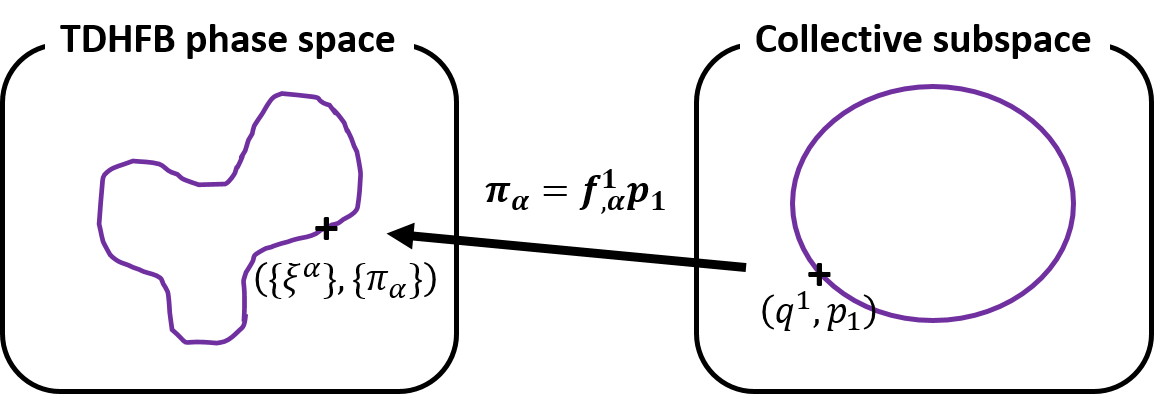
\includegraphics[width=80mm, bb=0 0 550 180]{SPA.png}
% \end{center}
%  \caption{For a TDHFB trajectory, the correspondence between TDHFB phase space and collective subspace.}
%  \label{fig:correspondence}
%\end{figure}
%We try to combine SPA with ASCC. The key point is to find the correspondence between TDHFB phase space and collective subspace in a TDHFB trajectory (See Fig. \ref{fig:correspondence}). We consider the time-dependent state vector $\ket{Z(t)}$ is in a collective subspace. With pairing correlation, $\ket{Z(t)}$ can be expressed as


\subsubsection{Notation and practical procedure for quantization}
\label{sec:notation}

For application of the ASCC+SPA method to the pairing model in Sec.~\ref{sec3},
we summarize some notations and procedures to obtain quantized states.

In Sec.~\ref{sec3}, the time-dependent generalized Slater determinants
(coherent states) are written as $\ket{Z}$ with complex variables
$Z_\alpha(t)$.
The variables $Z_\alpha$ are transformed into real variables
$(j^\alpha, -\chi_\alpha)$ that correspond to $(\xi^\alpha,\pi_\alpha)$
in Sec.~\ref{sec2}.
$\chi_\alpha$ and $j^\alpha$ correspond to
the ``angle'' and the ``number'' variables, respectively.
Although it is customary to take the angle as a coordinate,
since the angle $\chi_\alpha$ is time-odd quantities, 
we switch the coordinates and the momenta with minus signs
in front of variables $\chi$.
Similarly, the gauge angle $\Phi$ and the total particle number $J$
correspond to variables of the pair rotation, $-p_n$ and $q^n$, respectively.
%The collective variables $(q^1,p_1)$ in Sec.~\ref{sec2} are
%written as $(q,p)$ in Sec.~\ref{sec3} for simplicity.


%\begin{align}
% \ket{Z(t)} &= \ket{\Phi,J;q,p} = e^{-i\Phi \hat{J}} \ket{J;q,p} ,
% \label{GCS}
%\end{align}
%where $\Phi$ is the total gauge angle and $J=N/2$ is the conjugate momentum corresponding total particle number. The second equal sign indicates an intrinsic state $\ket{J;q,p}$ rotates in the gauge space. Since $[H,J]=0$, the classical Hamiltonian 
%becomes
%\begin{align}
% \mathcal{H} &= \braket{\Phi,J;q,p|H|\Phi,J;q,p} \nonumber \\
% &= \braket{J;q,p|H|J;q,p} \equiv \mathcal{H}_J(q,p)
%\end{align}  
%has no dependence of $\Phi$. Therefore, the classical Hamiltonian is the function of $(q,p)$ in a fixed particle number system, and correspond to (\ref{coll}). From ASCC, we can obtain the static state vector at each point of $q$, namely $\ket{J;q,p=0}$. To construct $\ket{J;q,p}$, we use (\ref{momenta}) at $(q,p)$ which we want to know in the collective phase space. Usually, we are interested in the points $(q^{(k)},p^{(k)})$ at the $k$-th TDHFB trajectory. Such $k$-th TDHFB trajectory is obtained from EBK quantization condition ($k$: integer)
%\begin{align}
%	\mathcal{T}_\circ[Z^{(k)}]=&
%	\oint \braket{Z^{(k)}(t')| i\hbar\frac{\partial}{\partial t'} |Z^{(k)}(t')} dt' \nonumber \\
%	=& \oint p^{(k)} dq^{(k)} = 2k\pi .
%	\label{EBK}
%\end{align}

According to the EBK quantization rule (\ref{EBK}),
the ground state with $k=0$ corresponds to nothing but the HFB state
with a fixed particle number $J(=q^n)$.
For the $k$-th excited states, we perform the following calculations:
\begin{enumerate}
\item Obtain the 1D collective subspace with canonical variables $(q^1,p_1)$
	according to the ASCC in Sec.~\ref{sec:ASCC}.
\item Find a trajectory $(q^1(t),p_1(t))$ which satisfies
the $k$-th EBK quantization condition (\ref{EBK}).
\item Calculate the action integral (\ref{tau}) for the $k$-th trajectory.
\item Using Eq.~(\ref{SPA}), construct the $k$-th excited state.
\end{enumerate}
The ASCC provides the 2D collective subspace $(q^1,J)$
and the generalized coherent states $\ket{\Phi=0,J;q,p=0}$.
For finite values of momenta, we use Eq.~(\ref{momenta})
to obtain the state $\ket{\Phi,J;q,p}$.

%%%%%%%%%%%%%%%%%%%%%%%%%%%%%%%%%%%%%%%%%%%%

\section{Pairing model}
\label{sec3}

We study low-lying excited $0^+$ states
in multi-level pairing model by applying the ASCC+SPA.
The Hamiltonian of the pairing model is given in terms of
single-particle energies $\epsilon_l$ and the pairing strength $g$ as
\begin{align}
	H &= \sum_\alpha \epsilon_\alpha n_\alpha - g \sum_{\alpha,\beta} S_\alpha^+ S_{\beta}^- \nonumber \\
    &= \sum_\alpha\epsilon_\alpha(2S_\alpha^0+\Omega_\alpha) - g S^+ S^{-} ,
\end{align}
where we use the SU(2) quasi-spin operators,
$\boldsymbol{S}=\sum_\alpha \boldsymbol{S}_\alpha$, with
\begin{eqnarray}
        S_\alpha^0 &=& \frac{1}{2}(\sum_ma_{j_\alpha m}^{\dag}a_{j_\alpha m}-\Omega_\alpha) ,\\
        S_\alpha^{+} &=& \sum_{m>0}a_{j_\alpha m}^{\dag}a_{j_\alpha\overline{m}}^{\dag} ,
\quad   S_\alpha^{-} = S_\alpha^{+\dag} .
\end{eqnarray}
Each single-particle energy $\epsilon_\alpha$ possesses $(2\Omega_\alpha)$-fold
degeneracy ($\Omega_\alpha=j_\alpha+1/2$)
and $\sum_{m>0}$ indicates the summation over $m=1/2,3/2,\cdots,$
and $\Omega_\alpha-1/2$.
The occupation number of each level $\alpha$ is given by
$
\hat{n}_\alpha = \sum_m a^{\dag}_{j_\alpha m}a_{j_\alpha m}
=2S_\alpha^0+\Omega_\alpha
$.
The quasi-spin operators satisfy the commutation relations
\begin{equation}
  [S_\alpha^0,S_\beta^{\pm}] = \pm\delta_{\alpha\beta}S_{\alpha}^{\pm},
\quad [S_{\alpha}^{+},S_{\beta}^{-}] = 2\delta_{\alpha\beta}S_{\alpha}^{0} .
\end{equation}
The magnitude of quasi-spin for each level is
$S_\alpha=\frac{1}{2}(\Omega_\alpha-\nu_\alpha)$, where $\nu_\alpha$
is the seniority
quantum number, namely the number of unpaired particle at the level $\alpha$.
In the present study, we only consider seniority zero states with
$\nu=\sum_\alpha \nu_\alpha=0$.
The residual two-body interaction only consists of monopole pairing
interaction which couples two particles to zero angular momentum.
We obtain exact solutions either by solving Richardson equation
\cite{Richardson,Richardson2,Richardson3} or
by diagonalizing the Hamiltonian using the quasi-spin symmetry.


\subsection{Classical form of TDHFB Hamiltonian}

The time-dependent coherent state for the seniority $\nu=0$ states
($S_\alpha=\Omega_\alpha/2$) is constructed with
time-dependent complex variables $Z_\alpha(t)$, as
\begin{equation}
	\ket{Z(t)} = \prod_{\alpha} \left(1+|Z_\alpha(t)|^2\right)^{-\Omega_\alpha/2}
	\exp [Z_\alpha(t) S_\alpha^{+}] \ket{0}
 \label{coherent}
\end{equation}
where $\ket{0}$ is the vacuum (zero particle) state.
The TDHFB motion is given by the time dependence of $Z_\alpha(t)$.
In the SU(2) quasi-spin representation,
$\ket{0}=\prod_\alpha \ket{S_\alpha,-S_\alpha}$.
The coherent state $\ket{Z(t)}$ is a superposition of
states with different particle numbers
without unpaired particles.
%If $Z_l$ are all real,
In the present pairing model,
the coherent state is the same as the time-dependent BCS wave function
with $Z_\alpha(t)=v_\alpha(t)/u_\alpha(t)$,
where $(u_\alpha(t),v_\alpha(t))$ are the time-dependent BCS $u,v$ factors.

The TDHFB equation can be derived from the time-dependent variational
principle ($\hbar=1$), $\delta \mathcal{S} = 0$, where
\begin{equation}
%  \delta \int \braket{\phi(t)|i\frac{\partial}{\partial t}-H|\phi(t)}dt = 0 ,
	\mathcal{S}\equiv \int \mathcal{L}(t) dt =
	\int \braket{Z(t)|i\frac{\partial}{\partial t}-H|Z(t)}dt.
  \label{TDHFB}
\end{equation}
After transformation of the complex into real variables,
$Z_\alpha = \tan{\frac{\theta_\alpha}{2}}e^{-i\chi_\alpha}$
($0\leq\theta\leq\pi$),
the Lagrangian $\mathcal{L}$ and the expectation value of the Hamiltonian
are written as
\begin{equation}
\mathcal{L}(t) = \sum_\alpha \frac{\Omega_\alpha}{2}
	(1-\cos{\theta}_\alpha)\dot{\chi_\alpha} - \mathcal{H}(Z,Z^*) ,
\end{equation}
with
\begin{align}
	\mathcal{H}(Z,Z^*) &\equiv \braket{Z|H|Z}& \nonumber \\
	&= \sum_\alpha \epsilon_\alpha\Omega_\alpha(1- \cos{\theta}_\alpha)
	\nonumber \\
	&- \frac{g}{4}\sum_\alpha \Omega_\alpha [\Omega_\alpha(1-\cos^2{\theta}_\alpha)+(1-\cos{\theta}_\alpha)^2] \nonumber \\
	- \frac{g}{4}\sum_{\alpha\neq \beta} \Omega_{\alpha}\Omega_{\beta}&\sqrt{(1-\cos^2{\theta}_{\alpha})(1-\cos^2{\theta}_{\beta})}e^{-i(\chi_{\alpha}-\chi_{\beta})}   .
\label{TDHFB_Hamiltonian_2}
\end{align}
Choose $\chi_\alpha$ as canonical coordinates, their conjugate momenta
are given by
\begin{align}
  j^\alpha\equiv
	\frac{\partial\mathcal{L}}{\partial\dot{\chi}_\alpha}=\frac{\Omega_\alpha}{2}
	(1-\cos{\theta}_\alpha) .
\end{align}
$\chi_\alpha$ represent a kind of gauge angle of each level,
and $j^\alpha$ correspond to the occupation number of each level,
$2j^\alpha=\bra{Z} \hat{n}_\alpha\ket{Z}$. 
As we mention in Sec.~\ref{sec:notation},
we switch the coordinates and momenta,
$(\chi_\alpha,j^\alpha) \rightarrow (j^\alpha,-\chi_\alpha)$,
to make the coordinates time even.
%Therefore, the TDHFB Hamiltonian can be represented by canonical variables
%$\mathcal{H}(Z,Z^*) = \mathcal{H}(\{\chi_l\},\{j_l\})$, and 
The TDHFB equation is equivalent to the classical Hamilton's equation
\begin{equation}
	-\dot{\chi_\alpha} = -\frac{\partial\mathcal{H}}{\partial j^\alpha}, \quad
	\dot{j^\alpha} = \frac{\partial\mathcal{H}}{\partial (-\chi_\alpha)} .
\end{equation}


\subsection{Application of ASCC}

%In this subsection, we use ($\alpha, \beta, \cdots$) to describe the degrees of freedom instead of $l$ to synchronize the notation with in Sec. \ref{ASCC}. 
We construct a 2D collective subspace $\Sigma_2$ from ASCC theory.
%Because the first order with respect to $\chi_{\alpha}$ is zero in TDHFB Hamiltonian, we assume $j^{\alpha}$ as coordinates and $\chi_{\alpha}$ as conjugate momenta.  The canonical variables are $(j^{\alpha},-\chi_{\alpha})$ and fulfill $\{j^{\alpha},-\chi_{\beta}\}_{PB}=\delta^{\alpha}_{\beta}$. 
We expand the classical Hamiltonian up to second order with respect to
momenta, $-\chi_{\alpha}$. 
\begin{align}
  \mathcal{H}(j,\chi) \approx& V(j) + \frac{1}{2}B^{\alpha\beta}(j)\chi_{\alpha}\chi_{\beta},
\end{align}
where potential $V(j)$ and the reciprocal mass parameter
$B^{\alpha\beta}(j)$ are given as
\begin{align}
  V(j) =& \mathcal{H}(j,\chi=0) \nonumber \\
	=& \sum_{\alpha} 2\epsilon_{\alpha}j^{\alpha} - g\sum_{\alpha} \left( \Omega_{\alpha}j^{\alpha} - (j^{\alpha})^2 +\frac{(j^{\alpha})^2}{\Omega_{\alpha}} \right) \nonumber \\
  &- g\sum_{\alpha\ne \beta} \sqrt{j^{\alpha}j^{\beta}(\Omega_{\alpha}-j^{\alpha})(\Omega_{\beta}-j^{\beta})} 	
\end{align}
%\begin{align}
\begin{eqnarray}
&&B^{\alpha\beta}(j) = \left. \frac{\partial^2\mathcal{H}}{\partial\chi_{\alpha}\partial\chi_{\beta}} \right|_{\chi=0} \\
\label{mass}
&&=
	\begin{cases}
2g\sum_{\gamma\ne \alpha} \sqrt{j^{\gamma}j^{\alpha}(\Omega_{\gamma}-j^{\gamma})(\Omega_{\alpha}-j^{\alpha})}
		& \text{for $\alpha=\beta$} \\
-2g\sqrt{j^{\alpha}j^{\beta}(\Omega_{\alpha}-j^{\alpha})(\Omega_{\beta}-j^{\beta})}
		& \text{for $\alpha\ne\beta$}
	\end{cases} \nonumber
\end{eqnarray}
%\end{align}
We may apply the ASCC method in Sec. \ref{sec:ASCC}
by regarding $\xi\to j$ and $\pi\to-\chi$.

The TDHFB conserves the average total particle number $N$.
We adopt 
\begin{equation}
	J\equiv N/2=\sum_\alpha j^\alpha ,
  \label{J}
\end{equation}
as a coordinate $q^n$.
Since this is explicitly given as the expectation value of the particle
number operator, curvature quantities,
such as $f^n_{,\alpha\beta}$ and $f^{(1)n\alpha\beta}$,
are explicitly calculable.
On the other hand, the gauge angle $\Phi=-p_n$ is not given a priori.
Since the ASCC solution provides $g^\alpha_{,n}$ as an eigenvector of
Eq. (\ref{mfQRPA}),
we may construct it as Eq. (\ref{coll_momenta}) in the first order
in $\pi=-\chi$.
We confirm that the pairing rotation corresponds to an eigenvector
of Eq. (\ref{mfQRPA}) with the zero frequency $\omega^2=0$.

%With the properties of the constant of motion, we discuss the practical solution of ASCC in pairing model. If we ignore the higher order term $f^{(1)1\alpha\beta}$, we can practice local harmonic equation (LHE)
%\begin{align}
%  B^{\beta\gamma}V_{;\gamma\alpha}f^1_{,\beta}  &= \omega^2 f^1_{,\alpha},\hspace{2em} 
%  B^{\beta\gamma}V_{;\gamma\alpha}g^{\alpha}_{,1} = \omega^2 g^{\beta}_{,1},
%  \label{LHE}
%\end{align}
%which simplifies the moving-frame QRPA equation (\ref{mfQRPA}) by replacing $\tilde{B}^{\beta\gamma}$ into $B^{\beta\gamma}$. Under (\ref{LHE}), 

%%%%%% I guess this is automatic. Check %%%%%%%%
%To guarantee the state vectors $\ket{Z(q)}$ are in the same total gauge angle $\Phi(q)=-\frac{1}{L} p_1\sum_{\alpha} f^1_{,\alpha}=0$, we correct the eigenvectors by
%\begin{align}
%  f^1_{,\alpha} \to f^1_{,\alpha} - \frac{1}{L}\sum_{\beta} f^1_{,\beta} 
%  \label{f}
%\end{align}
%after solving (\ref{LHE}) at each point of $q$.

In the present pairing model, 
from Eq. (\ref{total_gauge}), we find $J$ does not dependent on $\chi$.
This means $f^{(1)n\alpha\beta}=0$ in Eq. (\ref{P}),
thus, $\tilde{B}^{\beta\gamma}=B^{\beta\gamma}$.
The second derivative of $J$ with respect to $j$ also vanishes,
which indicates $f^{I}_{,\gamma\beta}$ in Eq.~(\ref{M}) is zero. 
%It indicates the chemical potential $\lambda_I(q)$ is not necessary information to calculate the matrix element in moving-frame QRPA equation.
In the present model, it is easy to find an explicit expression
for the gauge angle $\Phi$.
\begin{align}
  \Phi = \frac{1}{L}\sum_{\alpha} \chi_{\alpha},
  \label{total_gauge}
\end{align}
where $L$ is the number of available shells $\alpha=1,\cdots,L$.
Its conjugate variable
${\partial\mathcal{L}}/{\partial\dot{\Phi}}$
is indeed given by $J$ of Eq. (\ref{J}).
Again, exchanging coordinate and momentum,
we have $q^n=J$ and $p_n=-\Phi$.

%We consider the treatment for the constant of motion in pairing model. In the TDHFB Hamiltonian, there is no dependence about the total gauge angle
%\begin{align}
%  J \equiv \frac{\partial\mathcal{L}}{\partial\dot{\Phi}}=\sum_{\alpha} j^{\alpha} = \frac{N}{2}
%\end{align}
%is conserved quantity. 


\subsection{Application of SPA}

After deriving the collective subspace states $\Sigma_2$, 
we perform the quantization according to the SPA in Sec.~\ref{sec:SPA}.
Calculating a trajectory in the $(q^1,p_1)$ space,
we can identify a series of states $\{\ket{\Phi,J;q^1(t),p_1(t)}\}$
on the trajectory,
in the form of Eq. (\ref{coherent})
with parameters $Z_\alpha$ given at $(\Phi,J,q^1,p_1)$ and $q^a=p_a=0$ for
$a\geq 3$.
%Due to $J$ is conserved quantity, the action integral can be divided into two terms
Since the variables$(\Phi,J)$ and $(q^1,p_1)$ are separable,
we may take closed trajectories independently in $(\Phi,J)$ and $(q^1,p_1)$
sectors, which we denote here as $C_\Phi$ and $C_1$, respectively.
The action integral is given by
\begin{align}
\mathcal{T}(\Phi,J;q^1,p_1)
&= \int_{C_\Phi} \braket{\Phi(t),J;q^1,p_1|i\frac{\partial}{\partial t}|\Phi(t),J;q^1,p_1} dt \nonumber \\
+ \int_{C_1} &\braket{\Phi,J;q^1(t),p_1(t)|i\frac{\partial}{\partial t}|\Phi,J;q^1(t),p_1(t)} dt
 \nonumber \\
	&=J\Phi + \int_{C_1} \sum_\alpha j^\alpha d\chi_\alpha
	\nonumber \\
	&\equiv \mathcal{T}_\Phi(J,\Phi) +\mathcal{T}_1(q^1,p_1;J) .
	\label{tau}
\end{align}
In fact, the gauge-angle dependence is formally given as
\begin{equation}
\ket{\Phi,J;q^1,p_1} = e^{-i\Phi \hat{N}/2} \ket{J;q^1,p_q} .
\end{equation}
Then, the action for the trajectory $C_1$ can be also expressed as
$\mathcal{T}(q^1,p_1;J)=
 \int_{C_1} \braket{J;q^1,p_1|i\frac{\partial}{\partial t}|J;q^1,p_1} dt$.
%\begin{align}
%  \mathcal{T}(\Phi,J;q,p) &= \mathcal{T}_{\rm intr}(t) + J\Phi, 
%\end{align}
%%where the intrinsic action integral $\mathcal{T}_{\rm intr}(t)$ becomes
%The important point is $\mathcal{T}_{\rm intr}(t) \ne \int p dq$ at each $t$. For closed TDHFB trajectory, only $\mathcal{T}_{\rm intr}(t)$ contributes to the excited states.

In the su(2) representation, the invariant measure is
\begin{align}
  d\mu(Z) &= \prod_\alpha \frac{\Omega_\alpha+1}{\pi} (1+|Z_\alpha|^2)^{-2} d{\rm Re}Z d{\rm Im}Z \nonumber \\
=& \prod_\alpha \frac{-(\Omega_\alpha+1)}{4\pi} d \cos{\theta_\alpha} d\chi_\alpha \nonumber \\
 =& \prod_\alpha \frac{1+\Omega_\alpha^{-1}}{2\pi} d\chi_\alpha dj^\alpha \nonumber \\
 =& \left[ \prod_\alpha \frac{1+\Omega_\alpha^{-1}}{2\pi} \right] d\Phi dJ dq^1 dp_1 %\nonumber \\
  \prod_a dq^a dp_a
% d\Phi dJ dq dp = d\Phi dJ dE dt 
	\label{dmu}
\end{align}
where $(q^a,p_a)$ are the intrinsic canonical variables
decoupled from the collective subspace $\Sigma_2$.
For the last equation in Eq. (\ref{dmu}),
we used the invariance of the phase space volume element
in canonical transformation.
%The part of the invariant measure which contributes to the excited states is
According to (\ref{dmu}),
the weight function $\rho(q,p)$ in Eq. (\ref{SPA}) is just a constant,
thus, treated as the normalization of the wave function.
%\begin{align}
%d\mu(\Phi,J;q,p) \propto d\Phi dJ dqdp = d\Phi dJ dE dt. 
%\end{align}
%Under EBK quantization condition (\ref{EBK}),

%derive the explicit form of excited states in (\ref{SPA}). From (\ref{GCS}) and (\ref{J}), the state vector $\ket{\Phi,J;q,p}$ becomes
%\begin{align}
%  \ket{\Phi,J;q,p} &= \sum_{\{j_l\}} e^{-i\Phi \sum_l j_l} \ket{J;q,p} .
%\end{align}
The coherent state $\ket{\Phi,J;q^1,p_1}=\ket{Z}$ is
expanded in the su(2) quasispin basis as
\begin{align}
\ket{Z} &= 
\sum_{\{m_\alpha\}} A_m(Z) \ket{\cdots;S_\alpha,-S_\alpha+m_\alpha,\cdots}, \nonumber\\
\end{align}
where the summation is taken over all possible combinations
of integer values of $\{ m_\alpha\}$.
\begin{align}
A_m(Z) =& \prod_\alpha 
\frac{Z_\alpha^{m_\alpha}}
	{\left(1+|Z_\alpha|^2\right)^{\Omega_\alpha/2}m_\alpha!}
\sqrt{\frac{(\Omega_\alpha)! m_\alpha!}{(\Omega_\alpha-m_\alpha)!}} \nonumber\\
 =& \prod_\alpha \left(\frac{1-\cos{\theta}_\alpha}{2}\right)^{m_\alpha/2}\left(\frac{1+\cos{\theta}_\alpha}{2}\right)^{(\Omega_\alpha-m_\alpha)/2}
  \nonumber \\
  &\times\sqrt{\frac{(\Omega_\alpha)!}{m_\alpha!(\Omega_\alpha-m_\alpha)!}} e^{-i m_\alpha\chi_\alpha}  ,
	\label{A_m}
\end{align}
where the lower index $m$ indicates a combination of $\{ m_\alpha \}$.
The integer numbers $m_\alpha$ correspond to the number of pairs
in the level $\alpha$.
%is in fixed gauge angle ($\Phi=0$).
%

Using Eq.~(\ref{A_m}),
now, the $k$-th excited state is calculated as
\begin{align}
\ket{\psi_k} \propto& \oint_{C_\Phi} d\Phi \oint_{C_1} dt
\ket{\Phi,J;q^1,p_1} e^{i\mathcal{T}(\Phi,J;q^1,p_1)}
 \nonumber \\
	=& \sum_{\{m_\alpha\}}
	\int_0^{2\pi} d\Phi e^{i(J-\sum_\alpha m_\alpha)\Phi} \nonumber \\
&\times \oint dt e^{i\mathcal{T}_1}(t) B_m (Z) \ket{\cdots;S_\alpha,-S_\alpha+m_\alpha,\cdots} \nonumber \\
 \equiv& \sum_{\{m_\alpha\}_J} C_m \ket{\cdots;S_\alpha,-S_\alpha+m_\alpha,\cdots}
 \label{SPA2}
\end{align}
where $B_m(Z)$ are indentical to $A_m$ in Eq.~(\ref{A_m}) but
replacing $\chi_\alpha$ by the relative angles
$\phi_\alpha\equiv\chi_\alpha-\Phi$.
The coefficients $C_m$ are
\begin{align}
C_m = \oint_{C_1} dt e^{i\mathcal{T}_1(t)} B_m(Z(t))
  \label{coef}
\end{align}
In the last line of Eq. (\ref{SPA2}), the summation is restricted to
$\{m_\alpha\}$ that satisfy $\sum_\alpha m_\alpha=J$.
It is easy to find that $J$ must be integer,
according to the quantization rule (\ref{EBK}) for the $(J,\Phi)$ sector.

The SPA for the ground state ($k=0$) is given by the stationary point
in the $(q^1,p_1)$ sector,
namely, the HFB state $\ket{\Phi,J;q,p}=e^{-i\Phi\hat{N}/2}\ket{\rm HFB}$.
Nevertheless, the rotational motion in $\Phi(t)$ is present,
which leads to the number quantization (projection).
Therefore, Eq.~(\ref{SPA2}) becomes
\begin{align}
	\ket{\psi_{g.s.}} \propto& \sum_{\{m_\alpha\}}
	\int_0^{2\pi} d\Phi e^{i(J-\sum_\alpha m_\alpha)\Phi}
	\ket{\rm HFB},  
	\label{SPA3}
\end{align}
which is identical to the wave function of the particle number projection for HFB state.

%%%%%%%%%%%%%%%%%%%%%%%%%%%%%%%%%%%%%%%%%%%

\section{Results}
\label{sec4}

%We apply ASCC+SPA to study the multi-level system in pairing model. 
In the pairing model in Sec.~\ref{sec3},
the number of TDHFB degrees of freedom equals that of single particle levels.
% including the constant of motion (pairing rotation). We consider various systems, two-level system, three-level system, and Pb isotope system in each subsection respectively. Next, we discuss the dynamics in non-integrable (more than three-level) system.  
Since there is a constant of motion, the particle number, in addition to
the energy, the system is integrable for one- and two-level models.
We first apply the ASCC+SPA method to an integrable two-level model,
then, to non-integrable multi-level models.


\subsection{Integrable case: Two-level pairing model}

The two-level pairing model corresponds to the 2D TDHFB system.
Explicitly separating the gauge angle $\Phi$ and
fixing the particle number $J$,
the 2D TDHFB is reduced to the 1D system,
with the relative angle $\phi\equiv \chi_2-\chi_1$ and the relative
occupation $j\equiv (j_2-j_1)/2$ as canonical variables.
In Ref.~\cite{NN18}, using the explicit transformation to these
separable variables,
we examined performance of the SPA requantization
for the two-level model.
In this section, we apply the ASCC+SPA method to the same model.
In other words, the ASCC method finds the transformation.

Here, we study the system with equal degeneracy,
$\Omega_1=\Omega_2=8$, 
the pairing strength $g/(\epsilon_2-\epsilon_1)=0.2$,
and the particle number $N=16$. 
The moving-frame QRPA produces the zero mode and another eigenvector
with finite frequency $\omega^2\neq 0$.
We follow the latter mode to construct the collective path.
In the ASCC calculation, we set the increment of the
collective coordinate, $dq=0.01$,
in units of $1/\sqrt{\epsilon_2-\epsilon_1}$.
We confirm that the pair rotation always has zero frequency
on the collective path.
On the obtained collective path, we calculate classical trajectory
for the Hamiltonian
\begin{equation}
\mathcal{H}_{\rm coll}(q^1,p_1;J)=\frac{1}{2} p_1^2 + V(q^1,J) ,
\end{equation}
with $J=N/2=8$.
Calculated trajectories, satisfying the EBK quantization condition
(\ref{EBK}) for the first and second excited states ($0_2^+$ and $0_3^+$),
are mapped onto the $(\phi,j)$ plane and
shown in Fig. \ref{fig:N16_traj}.
We also calculate the trajectories using explicit transformation
of variables to $(\Phi,J;\phi,j)$, which
are shown by dashed lines in Fig. \ref{fig:N16_traj}.
We call this ``TDHFB trajectories''.
Small deviation in large $\phi$ is due to the neglect of higher-order
terms in $\chi_\alpha$ in the ASCC.
In fact, if we calculate the trajectories in the variables
$(\Phi,J;\phi,j)$ using the Hamiltonian truncated up to the
second order in $\chi_\alpha$ (``ATDHFB trajectories''),
we obtain the solid lines in Fig. \ref{fig:N16_traj},
which perfectly agree with the ASCC trajectories.

The action integrals $\mathcal{T}(t)$ corresponding to
these closed trajectories are shown in Fig. \ref{fig:N16_tau}.
For the $0_2^+$ state,
all three calculations well agree
with each other, while we see small deviation between the full TDHFB
and the ASCC/ATDHFB calculations for the $0_3^+$ state.

The calculated wave functions for excited $0^+$ states 
are shown in Fig. \ref{fig:N16_occ}. 
We show the occupation probability which is decomposed 
into $2n$-particle-$2n$-hole components. 
The left end of the horizontal axis at $j=j_{\rm min}$
corresponds to a state with $(m_1,m_2)=(N/2,0)$ where all the particles
are in the lower level $\epsilon_1$.
The next at $j=j_{\rm min}+1$ corresponds to the one with
$(m_1,m_2)=(N-2/2,1)$, and so on.
The results from ATDHFB+SPA and ASCC+SPA are identical to each other
within numerical error, which well reproduces
the TDHFB+SPA calculation.
(How about exact cal.?)

%we can obtain the obvious collective path from ASCC.
%The dynamics is exactly identical with adiabatic TDHFB (ATDHFB). We confirm that whether ASCC is identical to one-dimensional ATDHFB, and compare the difference with TDHFB, in numerical calculation.
%
%In two-level system, the classical Hamiltonian in (\ref{TDHFB_Hamiltonian_2}) is
%\begin{align}
%\mathcal{H} 
%  =& \sum_{l=1,2} \epsilon_l\Omega_l(1- \cos{\theta}_l)& \nonumber \\ 
% &- \frac{g}{4}\sum_{l=1,2} \Omega_l [\Omega_l(1-\cos^2{\theta}_l)+(1-\cos{\theta}_l)^2] \nonumber \\
%- \frac{g}{2} \Omega_{1}\Omega_{2}&\sqrt{(1-\cos^2{\theta}_{l_1})(1-\cos^2{\theta}_{l_2})}\cos{(\chi_{2}-\chi_{1})}   .
%\end{align}
%If we define the canonical coordinate $\phi=\chi_2-\chi_1$, it attributes to one-dimensional system. The conjugate momentum is $j= \frac{\partial\mathcal{L}}{\partial\dot{\phi}} = \{\Omega_2(1-\cos{\theta}_2) - \Omega_1(1-\cos{\theta}_1)\}/4$. The ATDHFB indicates that the Hamiltonian can be expanded up to second order with respect to $\phi$
%\begin{align}
%  \mathcal{H}(\phi,j) &\approx V(j) + \frac{1}{2}B^{-1}(j)\phi^2,
%\end{align}
%where $V(j)=\mathcal{H}(\phi=0,j)$ and $B^{-1}(j)= \left. \frac{\partial^2\mathcal{H}}{\partial\phi^2} \right|_{\phi=0}$.
%We know that the BCS ground state corresponds to the potential minimum point with $\phi=0$. If the pairing correlation is strong enough to bind the excited states in the collective potential,  the adiabatic approximation is expected to be well because the states are localized in small $\phi$ region. 
%

\begin{figure}[thb]
 \begin{center}
   \includegraphics[height=0.45\textwidth,angle=-90]{N16X3p2trajectory.eps}
 \end{center}
\caption{Classical trajectories satisfying the EBK condition
(\ref{EBK}) with $k=1$ and 2 in the $(\phi,j)$ phase space.
%The domain of phase space is $-\pi\le\phi<\pi$, $-4\le j\le4$. 
Crosses, solid and dashed lines correspond to the results
of ASCC+SPA, ATDHFB+SPA, and TDHFB+SPA, respectively. 
For the ASCC+SPA trajectories, we plot the crosses
every ten(?) points of the calculation,
namely $\delta q=0.1/\sqrt{\epsilon_2-\epsilon_1}$.
}
\label{fig:N16_traj}
\end{figure}
\begin{figure}[thb]
 \begin{center}
   \includegraphics[height=0.5\textwidth,angle=-90]{N16X3p2action.eps}
 \end{center}
\caption{Calculated action integrals for the $\ket{0_2^+}$ and $\ket{0_3^+}$ states as functions of time $t$.
Crosses, solid and dashed lines correspond to the ASCC+SPA,
the ATDHFB+SPA, and the TDHFB+SPA, respectively. 
%Dotted lines are the values correspond to EBK quantization condition for $\ket{0_2^+}$ and $\ket{0_3^+}$. 
We calculated the action integrals on each trajectory
from $(\phi,j)=(0,j_{\rm max})$ in the clockwise direction
in Fig. \ref{fig:N16_traj}.
}
\label{fig:N16_tau}
\end{figure}
\begin{figure}[thb]
 \begin{center}
   \includegraphics[height=0.5\textwidth,angle=-90]{N16X3p2occ.eps}
 \end{center}
\caption{
Occupation probabilities for the $0_2^+$ and $0_3^+$ states.
The horizontal line indicates the $m_2-m_1$ of the quasi-spin basis
in Eq. (\ref{SPA2}).
The vertical bars at each $m_2-m_1$
represent the ASCC+SPA, ATDHFB+SPA and TDHFB+SPA calculations,
respectively, from left to right.
}
 \label{fig:N16_occ}
\end{figure}


Comparing with the full TDHFB calculation with the ASCC+SPA approach
in the two-level pairing model,
we conclude that the ASCC is reliable for description of low-lying
collective states, for which the adiabatic approximation is justifiable.
In addition, the pair rotation is properly separated.
%we succeed to describe the bound collective excited states by ASCC+SPA. For the bound states, whether the adiabatic approximation included or not hardly has influence. Even for the weakly bound states, the adiabatic approximation is reasonable approximation.


\subsection{Non-integrable case (1): Three-level pairing model}
\label{sec:three-level-model}

In contrast to the two-level model,
the TDHFB for the three-level model is non-integrable.
%The simplest non-integrable system is three-level system. We have one trivial motion and two time-dependent degrees of freedom. 
We set parameters of the system as follows:
$\Omega_1=\Omega_2=\Omega_3=\Omega=\Omega=8$,
$\epsilon_1=-\epsilon_0$, $\epsilon_2=0$, $\epsilon_3=1.5\epsilon_0$,
and $g=0.2\epsilon_0$.
We use the parameter $\epsilon_0$ as the unit energy.
For the sub-shell closed configuration of $N=2\Omega=16$,
the HFB ground state changes from the normal phase to
the superfluid phase at $g_c=0.058\epsilon_0$.
We calculate a chain of systems with even particle number
from $N=14$ to $N=24$. 

We obtain three eigen-frequencies for the moving-frame QRPA equation, 
on the collective path (Fig. \ref{omega_sq}). 
First of all, we clearly identify the zero mode with $\omega^2=0$
everywhere along the collective path.
This means that the pair rotation is separated from the other
degrees of freedom in the ASCC.
The frequency could become imaginary ($\omega^2<0$).
Except for the case of sub-shell closure ($N=2\Omega_1=16$),
the frequency rapidly increases near the end points.
The end points are given by points where search for the next point
on the collective path in Sec.~\ref{sec:ASCC} fails.

We choose the lowest mode, except for the zero mode,
as a generator for the collective path ($q^1$).
Figure~\ref{occ_number} shows variation of the occupation probability
of each single-particle state, as functions of the collective
coordinate $q^1$ on the collective path.
The most striking feature is that the collective path is terminates
with special configurations which are given by the integer number
of occupation.
This is a reason why the search for the collective path fails
at the both ends.
The occupation of the level 3 ($\epsilon_3$) vanishes, while
those of the levels 1 and 2 become either maximum or minimum.
The left end of each panel in Fig.~\ref{occ_number} corresponds to 
a kind of ``Hartree-Fock'' state which minimizes
the single-particle-energiy sum, $\sum_\alpha 2j_\alpha \epsilon_\alpha$.
The pairing correlation is weakened in both ends of the
collective path.

The collective mass with respect to the coordinate $q^1$ is normalized
to unity.
The collective potential is shown in Fig.~\ref{potential}.
The range of $q^1$ is the largest for the system with $N=16$.
This is because the varition of $j^1$ and $j^2$ is the largest in
this case.

\begin{figure*}[t]
 \begin{center}
  \includegraphics[width=40mm,angle=-90]{omega_sq.eps}
 \end{center}
	\caption{Eigenvalues of moving-frame QRPA equation with respect to the collective coordinate $q$, from $N=14$ to $N=24$. Purple lines are spurious modes and green lines are chosen modes corresponding to the collective coordinate. In each panel, both edges correspond to the end points of the collective coordinate.
}
 \label{omega_sq}
\end{figure*}
\begin{figure*}[t]
 \begin{center}
  \includegraphics[width=40mm,angle=-90]{occ_number.eps}
 \end{center}
	\caption{Occupation numbers in each single-particle level with respect to the collective coordinate $q$, from $N=14$ to $N=24$. At the left end point of the collective coordinate in each panel, the configurations correspond to Hartree-Fock (HF) states.
}
 \label{occ_number}
\end{figure*}
\begin{figure}[htbp]
 \begin{center}
  \includegraphics[width=60mm,angle=-90]{potential.eps}
 \end{center}
	\caption{Collective potential obtained from ASCC. We adjusted the energy minimum point as $V=0$.
}
 \label{potential}
\end{figure}

Based on the collective path determined by the ASCC calculation,
we perform the requantization according to the SPA.
Table \ref{ex} shows the excitation energies of the first and the second
excited states, determined by the EBK quantization condition (\ref{EBK}).
Comparing the result of the ASCC+SPA with those of the exact calculation,
we find the excitation energies are reasonably well reproduced. 
The ASCC+SPA underestimates the excitation energies by about 5 \%.
%The difference is that the values from ASCC+SPA are 
%about $5\%$ smaller than exact solution. 

It should be noted that the second excited state in the collective path
corresponds to the $0_4^+$ state,
not to the $0_3^+$ state, in the exact calculation. 
We examine the interband $(k\neq k')$ pair addition transition,
\begin{equation}
B(P_{\rm ad};k\rightarrow k') \equiv 
	\left|\bra{0_{k'}^+;N+2} S^+ \ket{0_k^+;N}\right|^2 ,
\label{BPad}
\end{equation}
in the exact solution.
$B(P_{\rm ad};0_2^+\rightarrow 0_3^+)$ 
is $10\sim100$ times smaller than $B(P_{\rm ad};0_1^+\rightarrow 0_3^+)$,
while $B(P_{\rm ad};0_1^+\rightarrow 0_2^+)$ and
$B(P_{\rm ad};0_1^+\rightarrow 0_3^+)$ are in the same order.
The ASCC+SPA produces states in the same family,
namely, those belonging to the same collective subspace (path).
In the phonon-like picture,
we expect similar magnitude of strengths for
$B(P_{\rm ad};{\rm g.s.}\rightarrow \omega_{\rm phon})$
and
$B(P_{\rm ad};\omega_{\rm phon}\rightarrow 2\omega_{\rm phon})$,
but smaller values of
$B(P_{\rm ad};{\rm g.s.}\rightarrow 2\omega_{\rm phon})$.
Thus, the $0_4^+$ state in the exact calculation
corresponds to the two-phonon state in the ASCC+SPA.
The $0_3^+$ state in the exact calculation may correspond to
a collective path associated with another solution of the moving-frame QRPA
(thin black line in Fig.~\ref{omega_sq}).

%It indicates that $\ket{0_3^+}$ is also one-phonon state which belongs to the other collective path (black line in Fig. \ref{omega_sq}). About two-phonon states, we can easily find the candidates of two-phonon states from excitation energies and $B(P_{\rm ad};0_1^+\rightarrow 0_{ex}^+)$. In the candidates, $\ket{0_4^+}$ is the lowest two-phonon state and $B(P_{\rm ad};0_2^+\rightarrow 0_4^+)$ is much larger than $B(P_{\rm ad};0_3^+\rightarrow 0_4^+)$. Therefore, $\ket{0_4^+}$ is considered to be most appropriate corresponding to the second excited state in ASCC+SPA calculation.

Next, we calculate the wave functions,
according to Eqs.~(\ref{SPA2}) and (\ref{SPA3}).
The ground state corresponds to the number-projected HFB state
(variation before projection).
In contrast, excited states are given as superposition of
generalized Slater determinants in the collective subspace,
Using these wave function of excited states, 
the pair addition transition strengths
are shown in Fig. \ref{3levelPad}.
For the intraband transition ($k=k'$ in Eq. (\ref{BPad})),
the ASCC+SPA method well reproduces the strengths of the exact calculation.
The ground-to-ground transitions, $B(P_{\rm ad};0_1^+\rightarrow 0_1^+)$
are perfectly reproduced, while
$B(P_{\rm ad};0_2^+\rightarrow 0_2^+)$ are underestimated 
by about $10\%\sim20\%$.

It is more difficult to reproduce the absolute magnitude of
interband transitions ($k\neq k'$), 
which are far smaller than the intraband transitions.
Although the increasing (decreasing) trend for
$B(P_{\rm ad};0_2^+\rightarrow 0_1^+)$
($B(P_{\rm ad};0_1^+\rightarrow 0_2^+)$)
as a function of the particle number is properly reproduced,
the absolute magnitude is signiicantely underestimated in the ASCC+SPA.
This is due to extremely small collectivity in the interband transitions.
Almost all the strengths are absorbed in the intraband transitions.
Even in the exact calculation, the pair addition strength is
about two orders of magnitude smaller than the intraband strength.
Remember that the non-collective limit ($g\rightarrow 0$) of this
value is $B(P_{\rm ad};0_1^+\rightarrow 0_2^+)=\Omega$.
Therefore, the pairing correlation hinders the interband transitions
by about one order of magnitude.
For such tiny quantities, perhaps, 
the reduction to the 1D collective path is not well justified.
%In our previous study on the two-level case, we found that
%the SPA reasonably well reproduces interband transitions \cite{NN18}.
%The present case corresponds to a strong pairing case with
%the strongly hindered interband transitions.


%It is difficult to reproduce the absolute value of exact solution.
%However, because the pairing correlation is enough strong in this case, the strength of intraband transition is dominant compared with interband transition.
%We can find that 
%$B(P_{\rm ad};0_1^+\rightarrow 0_2^+)$ and $B(P_{\rm ad};0_2^+\rightarrow 0_1^+)$ are only about $1\%$ of $B(P_{\rm ad};0_1^+\rightarrow 0_1^+)$ and $B(P_{\rm ad};0_2^+\rightarrow 0_2^+)$. Therefore, the interband transition can be regarded as reasonable. From all above results, we can conclude that ASCC+SPA reproduces exact solution quantitatively. 

We should remark here that there is a difficulty in the present ASCC+SPA
requantization for weak paring cases.
In such cases, the potential minimum is close to the left end 
($q^1=q_L$) of the collective path, and the potential height
at $q^1=q_L$, $V(q_L) - V(0)$, becomes small.
Then, a classical trajectory at $E>V(q_L)$ hit this boundary ($q^1=q_L$).
In construction of wave functions,
the boundary condition at $q^1=q_L$ significantly influences the result.
In the present study, we choose a strong pairing case to avoid
such a situation.
As in Feb.~\ref{potential}, the potential height at $q^1=q_L$ has
about $10\epsilon_0$ which is larger than the excitation energies
of the second excitation.
Therefore, all the trajectories are ``closed'' in the usual sense.

%We skipped the result about $\ket{0_3^+}$.
\begin{table}[htbp]
\begin{ruledtabular}
\begin{tabular}{c|cccccc}
            $N$ & $14$ & $16$ & $18$ & $20$ & $22$ & $24$\\ \hline
ASCC+SPA (1st exc.) & $3.87$ & $3.90$ & $3.97$ & $4.09$ & $4.23$ & $4.33$\\
    Exact & $4.09$ & $4.13$ & $4.20$ & $4.30$ & $4.44$ & $4.60$\\ \hline
ASCC+SPA (2nd exc.)& $7.42$ & $7.42$ & $7.60$ & $7.92$ & $8.26$ & $8.47$\\
Exact & $7.65$ & $7.71$ & $7.88$ & $8.15$ & $8.49$ & $8.74$
\end{tabular}
\end{ruledtabular}
\caption{Calculated excitation energies of the first and the second
excited states in units of $\epsilon_0$.
In the exact calculation, the second excited state in the ASCC+SPA
corresponds to the $0_4^+$ state.
See text for details.}
\label{ex}
\end{table}

\begin{figure}[htbp]
 \begin{center}
  \includegraphics[width=60mm,angle=-90]{intra_trans.eps}
 \end{center}
 \begin{center}
  \includegraphics[width=60mm,angle=-90]{inter_trans.eps}
 \end{center}
\caption{Calculated strength of pair-addition transition (\ref{BPad})
from $N=14$ to $N=22$. 
The solid (dashed) lines correspond to the ASCC+SPA (exact) calculation.
The horizontal line indicates the particle number of the initial states.
The upper panel shows the intraband transitions,
$\ket{0_1^+}\to\ket{0_1^+}$ and $\ket{0_2^+}\to\ket{0_2^+}$,
while lower panel shows the interband transitions,
$\ket{0_1^+}\to\ket{0_2^+}$ and $\ket{0_2^+}\to\ket{0_1^+}$.
}
 \label{3levelPad}
\end{figure}




\subsection{Non-integrable case (2): Pb isotopes}
\label{sec:Pb_isotopes}

Finally, we apply our method to neutrons' pairing dynamics in 
neutron-deficient Pb isotopes.
The spherical single-particle levels of neutrons
between the magic number 82 and 126 are adopted and
their energies are presented in Table \ref{Pb}. 
The coupling constant $g=0.138$ MeV is determined to reproduce
the experimental pairing gap given by the even-odd mass difference,
$\Delta(N)=\frac{(-1)^{N+1}}{2}(B(N+1)-2B(N)+B(N-1))$ of ${}^{192}$Pb.
The even-even nuclei from ${}^{188}$Pb to ${}^{194}$Pb
are studied.
\begin{table}[htbp]
\begin{ruledtabular}
\begin{tabular}{c|cccccc}
  orbit& $h_{9/2}$ & $f_{7/2}$ & $i_{13/2}$ & $p_{3/2}$ & $f_{5/2}$ & $p_{1/2}$\\ \hline
  energy(MeV)& $-10.94$ & $-10.69$ & $-8.74$ & $-8.44$ & $-8.16$ & $-7.45$\\
\end{tabular}
\end{ruledtabular}
\caption{Single-particle energies of Pb isotopes used in the calculation
in units of MeV.
These are obtained from spherical Woods-Saxon potential
with the universal parameters(?) \cite{??}. }
\label{Pb}
\end{table}

The TDHFB dynamics is described by six degrees of freedom.
Figure \ref{Pb_omega_sq} shows eigenvalues of the
moving-frame QRPA equation.
Again, we find that there is a zero mode corresponding to
the neutron pair rotation.
Among the five vibrational modes, we choose the lowest one to
construct the collective path in the ASCC.
This lowest mode never crosses with other modes,
though the spacing between the lowest to the next lowest mode
can be very small, especially for ${}^{194}$Pb.
The evolution of the occupation numbers along the collective path
is shown in Fig. \ref{Pb_occ_number}.
Similarly to the three-level model, 
the end points of the collective path indicate exactly
the integer numbers, and
the left end of each panel corresponds to the ``HF''-like state.
On the collective path, the occupation of $i_{13/2}$, $p_{3/2}$, and
$f_{5/2}$ mainly changes.
%The last neutrons are in $i_{13/2}$ from ${}^{188}$Pb to ${}^{194}$Pb. 

The collective potentials for these isotopes are shown
in Fig. \ref{Pb_potential}.
The heights of the potentials at the left end, $V(q_L)-V(0)$,
are $2\sim3.5$ MeV.
For $^{186}$Pb, the height of the potential is not
enough to satisfy the condition, $E<V(q_L)$,
to have a closed trajectory for the first excited state
(See the last paragraph in Sec.~\ref{sec:three-level-model}).
We encounter another kind of problem for $^{196}$Pb,
which will be discussed in Sec.~\ref{sec5}.
Therefore, in this paper, we calculate the first excited states
in $^{188,190,192,194}$Pb.

\begin{figure*}[t]
 \begin{center}
  \includegraphics[width=40mm,angle=-90]{Pbomega_sq.eps}
 \end{center}
	\caption{The same as Fig. \ref{omega_sq} but for Pb isotopes.
}
 \label{Pb_omega_sq}
\end{figure*}
\begin{figure*}[t]
 \begin{center}
  \includegraphics[width=40mm,angle=-90]{Pbocc_number.eps}
 \end{center}
	\caption{The same as Fig. \ref{occ_number} but for Pb isotopes.
}
 \label{Pb_occ_number}
\end{figure*}
\begin{figure}[htbp]
 \begin{center}
  \includegraphics[width=60mm,angle=-90]{Pbpotential.eps}
 \end{center}
	\caption{The same as Fig. \ref{potential} but for Pb isotopes.
}
 \label{Pb_potential}
\end{figure}

We show the calculated excitation energy of the first excited state
in Table~\ref{Pb}.
Experimentally, this pairing vibrational excited $0^+$ state is
fragmented into several $0^+$ states due to other correlations,
such as quadrupole correlation, not taken into account in the present model.
%The value is nothing to do with experimental value because pairing model is too simple to describe realistic nuclear interaction. 
We make a comparison with the exact solution of the multi-level
pairing model.
The ASCC+SPA method quantitatively reproduces the excitation energy of
the exact solution.

The pair-addition transition strengths are shown in Fig. \ref{PbPad}.
The feature similar to the three-level case is observed;
dominant intraband transition and very weak interband transitions.
the accuracy from 
The ASCC+SPA method well reproduces
$B(P_{\rm ad};0_1^+\rightarrow 0_1^+)$,
and qualitatively reproduces
$B(P_{\rm ad};0_2^+\rightarrow 0_2^+)$ as well.
The deviation for the latter is about $25\%$.
The interband transitions are smaller than the intraband transitions
by more than two orders of magnitude.
This is also similar to the three-level model discussed
in Sec.~\ref{sec:three-level-model}.
For such weak transitions, the ASCC+SPA significantly
underestimates the strengths.
We may say that the ASCC+SPA gives reasonable results for the intraband
transitions in realistic values of pairing coupling constant $g$ and
single-particle levels.

\begin{table}[htbp]
\begin{ruledtabular}
\begin{tabular}{c|cccccc}
   & ${}^{186}$Pb & ${}^{188}$Pb & ${}^{190}$Pb & ${}^{192}$Pb & ${}^{194}$Pb & ${}^{196}$Pb\\ \hline
ASCC+SPA & $-$ & $2.31$ & $2.21$ & $2.12$ & $2.04$ & $-$ \\ 
Exact & $2.58$ & $2.44$ & $2.34$ & $2.25$ & $2.20$ & $2.15$
\end{tabular}
\end{ruledtabular}
\caption{The same as Table. \ref{ex} but for Pb isotopes. The energies are given in units of MeV.}
\label{Pb_ex}
\end{table}
\begin{figure}[htbp]
 \begin{center}
  \includegraphics[width=60mm,angle=-90]{Pbintra_trans.eps}
 \end{center}
 \begin{center}
  \includegraphics[width=60mm,angle=-90]{Pbinter_trans.eps}
 \end{center}
	\caption{The same as Fig. \ref{3levelPad} but for Pb isotopes.
}
 \label{PbPad}
\end{figure}

Finally, we discuss the validity of the collective model approach
assuming the pairing gap as a collective coordinate.
The 5D collective Hamiltonian assuming the quadrupole deformation
parameters $\alpha_{2\mu} (\mu=\pm2,\pm1,0)$ as the collective coordinates
is widely utilized to analyze experimental data of quadrupole states.
Similarly, we may construct the pairing collective Hamiltonian
in terms of the pairing gap $\Delta$ and the gauge angle $\Phi$. 
As far as there is one-to-one correspondence between $\Delta$ 
and the collective variable $q^1$ we obtained in the present study,
we can transform the collective Hamiltonian in $(q^1,\Phi)$
into the one in $(\Delta,\Phi)$.
The pairing gap $\Delta$ is defined as
\begin{align}
  \Delta (q) &\equiv \left. g\braket{\Phi,J;q,p|S^-|\Phi,J;q,p} \right|_{\Phi=p=0} \nonumber \\
  &= g\sum_\alpha \sqrt{j^\alpha(\Omega_\alpha-j^\alpha)} .
\end{align}
Figure \ref{192Pb_gap} shows the pairing gap $\Delta$ in ${}^{192}$Pb
as a function of the collective coordinate $q^1$.
The peak in $\Delta$ is near $q^1=0$ and it is not a monotonic
function of $q^1$, thus, no one-to-one correspondence exists.
The same behavior is observed for other Pb isotopes too.
Therefore, the pairing gap $\Delta$ is not suitable collective coordinate
to describe the pairing dynamics in the multi-level model.

%Because only one orbit near the Fermi energy ($i_{13/2}$ orbit for both end points) contributes the value of pairing gap, the value at both end points are small compared with the value around the ground state. There is no one-to-one correspondence between $\Delta$ and $q$ not only in ${}^{192}$Pb, but also in all multi-level systems. 


%As with the 5D collective model, pairing can also be supposed as a sort of deformation. The collective model is described by
%the pair deformation parameters pairing gap $\Delta$ and global gauge angle $\Phi$. 
%The utilization of the collective model for nuclear pairing dynamics was done in several references\cite{??}. In our previous study, however, we find that the pairing gap $\Delta$ is not proper to be the collective coordinate in two-level pairing model \cite{??}. In multi-level system, we can investigate the relations between the pairing gap and the collective coordinate. 

\begin{figure}[htbp]
 \begin{center}
  \includegraphics[width=60mm,angle=-90]{192Pbgap.eps}
 \end{center}
	\caption{Pairing gap as a function of collective coordinate in ${}^{192}$Pb. 
}
 \label{192Pb_gap}
\end{figure}

%%%%%%%%%%%%%%%%%%%%%%%%%%%%%%%%%%%%%%%%%

\section{Conclusion and discussion}
\label{sec5}

Extending our former work \cite{NN18},
which demonstrated the accuracy of SPA for the requantization
of TDHFB dynamics in the two-level pairing model, 
we propose the ASCC+SPA method for non-integrable systems.
In this approach, we use the ASCC method to extract the 2D
collective subspace including the pair rotation.
In other words, we map the non-integrable system to an approximate
integrable system described by $(q^1,p_1;J,\Phi)$.

%to extend SPA into non-integrable system is to combine with ASCC. We constructed the theoretical framework of ASCC+SPA for bound states, which is bound in the collective potential from ASCC. 
%Besides the collective Hamiltonian, $Q$ operator at each point of collective path is also necessary input information.

We apply the ASCC+SPA method to the multi-level pairing model.
%Because the gauge angle $\Phi$ is a cyclic variable, 
%the simplest non-integrable system is three level system. 
We investigate the three-level model and 
the multi-level model simulating Pb isotopes
with realistic pairing coupling constant $g$ and single-particle levels.
In both cases, the low-lying excited $0^+$ states obtained with
the ASCC+SPA well reproduce the exact solutions
not only of excitation energies but also of wave functions.
In the ASCC+SPA, the pair-transition calculation is straightforward,
because we have a microscopic wave function for every quantized state.
This overcomes a disadvantage in the conventional canonical requantization
in which we need to construct the pair-transition operator
in terms of the collective variables only.

Although the overall agreement between the ASCC+SPA and the exact
calculations is good in general,
we have encountered several problems remaining to be solved.
First, we can calculate a classical trajectory bound by the
pocket of a potential, however, it is not trivial how to treat
``unbound'' trajectories that hit the end point of the collective path.
See the potentials in Figs. \ref{potential} and \ref{Pb_potential}.
This happens in the calculation of ${}^{186}$Pb
(Sec.~\ref{sec:Pb_isotopes}).
Probably, it is necessary to find a proper boundary condition
in the collective subspace.
For instance, the 5D quadrupole collective model has
such boundary conditions imposed by the symmetry property of
the quadrupole degrees of freedom \cite{KB67}.

The second problem occured in the calculation of $^{196}$Pb,
in which we have encountered complex eigenvalues and eigenvectors
of the moving-frame QRPA equation.
This happens at a point where the two eigenenegies become
identical, $\omega_1^2=\omega_2^2$, namely at a crossing point.
We do not have a problem for the crossing between the pair rotational
mode and the other modes.
Currently, we do not know exactly when the complex solutions emerge.

Another problem we need to solve is a description of the
quantum tunneling.
The tunneling plays an essential role in
spontaneous fission, sub-barrier fusion reaction, and
shape coexistence phenomena \cite{NMMY16,WN16,WN17,HNMM07,HNMM08}.
In the present ASCC+SPA, the classical trajectory
cannot penetrate the potential barrier.
Since the ASCC is able to provide the 1D collective coordinate,
the imaginary-time TDHF is feasible and may be a solution
to this problem \cite{Neg82}.
These remaining issues in the ASCC+SPA approach should be
addressed in future.

%The crossing of the eigenvalues from the moving-frame QRPA equation
%in the collective path.
%No problem occurs when two completely orthogonal modes crossing, such as rotational mode and vibrational mode (e.g. N=14,16,18,20 in Fig. \ref{omega_sq}).
%However, if two vibrational modes not orthogonal with each other become the same eigenvalues, the ASCC calculation stops.
%Actually, the two eigenvalues become complex conjugate values and the next mesh point of collective path cannot be decided properly. Such case is occurred in ${}^{196}$Pb.
%The eigenvalues crossing problem supposed to be the rare case because ${}^{196}$Pb system is the only case including the previous studies about the application of ASCC.

%The difficulty for the application to the unbound states is that the wave function from SPA is not stationary state because the classical trajectory in phase space is not periodic.


\begin{acknowledgments}
This work is supported in part by JSPS KAKENHI Grants No. ????
and
by JSPS-NSFC Bilateral Program for Joint Research Project
on Nuclear mass and life for unravelling mysteries of r-process.
Numerical calculations were performed in part using COMA at the CCS,
University of Tsukuba.
%and by ImPACT Program of Council for Science,
%Technology and Innovation (Cabinet Office, Government of Japan).
\end{acknowledgments}

\bibliographystyle{apsrev4-1}
\bibliography{ref}

\end{document}

